%
% The first command in your LaTeX source must be the \documentclass command.
\documentclass[sigconf]{acmart}

% Disable the extra information at the foot at first page for better viewing experience for a normal document.
\settopmatter{printacmref=false} % Removes citation information below abstract
\renewcommand\footnotetextcopyrightpermission[1]{} % removes footnote with conference information in first column
\pagestyle{plain} % removes running headers

%
% defining the \BibTeX command - from Oren Patashnik's original BibTeX documentation.
\def\BibTeX{{\rm B\kern-.05em{\sc i\kern-.025em b}\kern-.08emT\kern-.1667em\lower.7ex\hbox{E}\kern-.125emX}}
    
% Rights management information. 
% This information is sent to you when you complete the rights form.
% These commands have SAMPLE values in them; it is your responsibility as an author to replace
% the commands and values with those provided to you when you complete the rights form.
%
% These commands are for a PROCEEDINGS abstract or paper.
%\copyrightyear{2018}
%\acmYear{2018}
%\setcopyright{acmlicensed}
%\acmConference[Woodstock '18]{Woodstock '18: ACM Symposium on Neural Gaze Detection}{June 03--05, 2018}{Woodstock, NY}
%\acmBooktitle{Woodstock '18: ACM Symposium on Neural Gaze Detection, June 03--05, 2018, Woodstock, NY}
%\acmPrice{15.00}
%\acmDOI{10.1145/1122445.1122456}
%\acmISBN{978-1-4503-9999-9/18/06}

%
% These commands are for a JOURNAL article.
%\setcopyright{acmcopyright}
%\acmJournal{TOG}
%\acmYear{2018}\acmVolume{37}\acmNumber{4}\acmArticle{111}\acmMonth{8}
%\acmDOI{10.1145/1122445.1122456}

%
% Submission ID. 
% Use this when submitting an article to a sponsored event. You'll receive a unique submission ID from the organizers
% of the event, and this ID should be used as the parameter to this command.
%\acmSubmissionID{123-A56-BU3}

%
% The majority of ACM publications use numbered citations and references. If you are preparing content for an event
% sponsored by ACM SIGGRAPH, you must use the "author year" style of citations and references. Uncommenting
% the next command will enable that style.
%\citestyle{acmauthoryear}

%
% end of the preamble, start of the body of the document source.
%\setcopyright{none}
\begin{document}

%
% The "title" command has an optional parameter, allowing the author to define a "short title" to be used in page headers.
\title{Paper Review CS846, Jan. 30\\
    {\it Aggregating empirical evidence for more trustworthy decisions} \\
    and {\it The truth, the whole truth, and nothing but the truth: A pragmatic guide to assessing empirical evaluation}
}

%
% The "author" command and its associated commands are used to define the authors and their affiliations.
% Of note is the shared affiliation of the first two authors, and the "authornote" and "authornotemark" commands
% used to denote shared contribution to the research.
\author{Wenhan Zhu (Cosmos)}
\email{w65zhu@uwaterloo.ca}
\affiliation{%
  \institution{University of Waterloo}
  \city{Waterloo}
  \country{Canada}
}

%
% The abstract is a short summary of the work to be presented in the article.
\begin{abstract}
    This week's chapter from the book being reviewed here is {\bf Aggregating empirical evidence for more trustworthy decisions} by {\it Donald Budgen} and {\bf The true, the whole true, and nothing but the true: A pragmatic guide to assessing empirical evaluation} by {\it Blackburn et al.}

    {\it Budgen}'s chapter is mainly about what makes an evidence to be true evidence and how can be make decisions based on systematic reviews created from the evidence and how exactly can we do it.

    {\it Blackburn et al.} talked about giving claims and evaluation of the claims and what can go wrong when doing so in the field of computer science in programming languages and system. They gave a very in depth description of claims and evaluation and how they work together to introduce new ideas to the field. They also proposed a vision to have more papers with either great evaluation or great novelty ideas to be considered by the community when submitting to conferences. 

\end{abstract}

%
% Keywords. The author(s) should pick words that accurately describe the work being
% presented. Separate the keywords with commas.
\keywords{paper review}

%
% A "teaser" image appears between the author and affiliation information and the body 
% of the document, and typically spans the page. 
%\begin{teaserfigure}
  %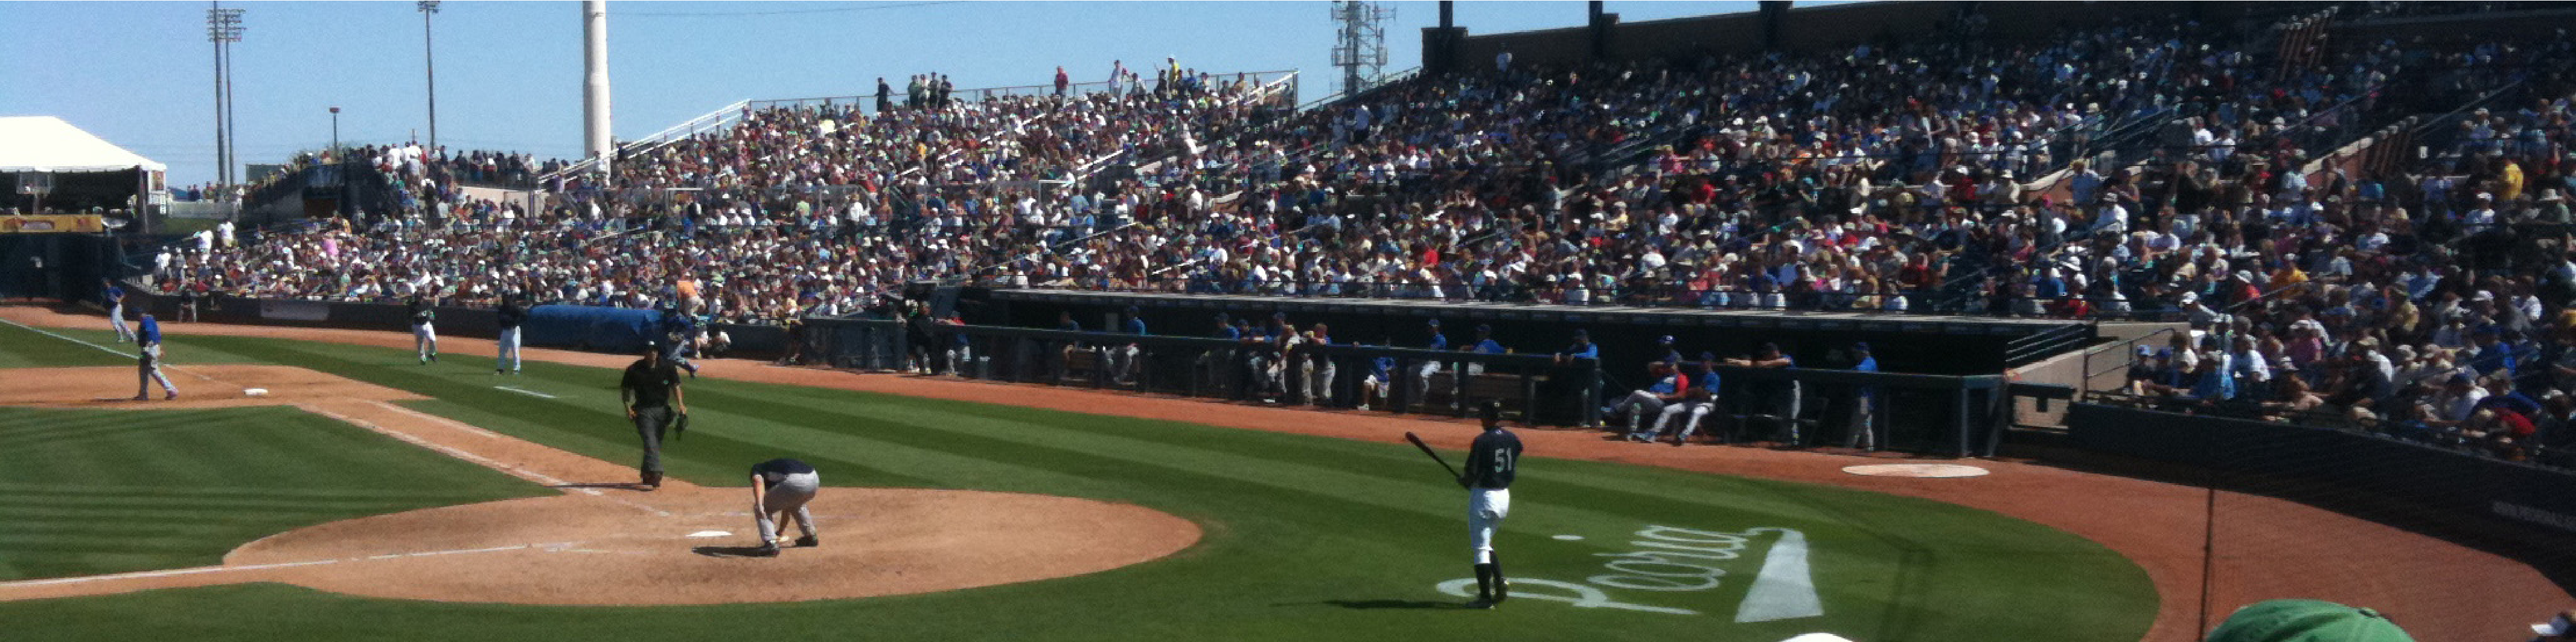
\includegraphics[width=\textwidth]{sampleteaser}
  %\caption{Seattle Mariners at Spring Training, 2010.}
  %\Description{Enjoying the baseball game from the third-base seats. Ichiro Suzuki preparing to bat.}
  %\label{fig:teaser}
%\end{teaserfigure}

%
% This command processes the author and affiliation and title information and builds
% the first part of the formatted document.
\maketitle

\section{Summary}

{\it Budgen} starts the chapter by using an example of when having pizza at one night and then had a bad dream later that night does not make having pizza an evidence of having the bad dream. However, when we are dealing with evidences in empirical software engineering, it's not that clear that whether one thing is the causation of the other or what is the evidence of something happening. In empirical studies, we need to take information from large number of human participants in order to make sure when repeating the study, variations will be small. When designing experiments, we want to take control of the independent variable however, it is not always true that we can achieve that. During the process, we also need to make decisions, but these decisions are not prune to bias. So evidence-based paradigm and systematic reviews are introduced as the 'model' for evidence-based decision-making. There are 5 steps of the process.

\begin{enumerate}
    \item Transform the information of some intervention to a question that can be answered.
    \item Determine the best evidence of the question by ways that are systematic, objective and unbiased.
    \item Critically evaluate the evidence from different points such as validity, impact and applicability.
    \item Find experts in the domain and have them evaluate it.
    \item Evaluate the results and use to improve the preceding steps.
\end{enumerate}

Steps 1-3 forms a systematic review. It is also considered as a secondary study since it aggregate results from other studies and does not involve the original participants. The original studies are primary studies. 

Despite, in original usage in medicine, when a doctor can give suggestion of which medicine to use base on systematic review. In the context of software engineering its often hard to make a decision. {\it Budgen} suggests it due to in the nature of medicine, the comparison are similar but in software engineering both the approach and evaluation might be different which makes gathering information during the systematic review hard. 

{\it Budgen} also mentioned just as many other methods in software engineering, systematic review is no 'silver bullet' solution.

{\it Blackburn et al.} gave a guide to assessing empirical evaluations. The paper talks about the process of empirical evaluation and categorized them by sins. In empirical evaluation, we have a claim and an evaluation of the claim. 

{\bf Sins of reasoning} happens when the scope of the claim does not align with the scope of the evaluation. If we consider the Venn diagram of claim and evaluation. We can denote the areas in three parts, A, B and C, where A is claim only, B is both claim and evaluation, and C is evaluation only. When A is empty and B, C are not, we have sin of ignorance where we evaluated the claim with data that was not originally in the claim. When C is empty and A, B are not, we suffer from sin of inappropriateness where we did not evaluate all of the claim. And when B is empty and A, C are not, the claim and the evaluation are disjoint, and it's the sin of inconsistency since we are sort of comparing apples and oranges. And when all are not empty, we suffer from both sin of ignorance and sin of inappropriateness.

{\bf Sins of exposition} can happen when the claim or evaluation does not convey it's ideas. Sin of inscrutability happens when the claim is not described adequately. It may happen when the author neglect part of the claim or the claim is ambiguous when it comes to wording. Since the claim is synthesized by it creator it should always be possible to make it clear. The sin of irreproducibility is a sin that happens when the evaluation is inadequate. It can happen when some of the evaluation phase is omitted either because of the author not knowing it's important or have to be removed due to constrains of length of work. When sins of exposition happens, people will not be able to figure out if the claim suffer from the sins of reasoning.

To avoid sin of inscrutability we can make our best effort to describe the claim as clear and as unambiguous as possible. To avoid sin of irreproducibility we should state all relevant control variables whether we believe they are related or not.

To avoid sin of ignorance and sin of inappropriateness, we should consider the methods we use in evaluation and make sure it's viable in our claims. Although it seems to be simple, in practice there are many factors that can go wrong. To avoid sin of inconsistency, we need to make sure that we are evaluating what we actually want to evaluation. The sins of reasoning all seems to be simple and obvious, however, due to the lack of knowledge in practice is much more harder than we think they are.

The authors suggested evaluations of claims in other fields such that repeating existing work and having a third party evaluation will help assessing empirical studies.

\section{Thoughts}
The chapter and the paper talked about how empirical studies should be looked at and how to avoid problems in this process. Different fields in science have developed different ways of dealing with empirical studies and software engineering borrow many ideas but they don't always works as the place where they borrowed.

When conducting an empirical study it is important to make sure we are not biased and both the evaluation and claim are as clear as possible and provide enough information so that the study can be repeated. During the process, the selection of method and the used data needs to fit and make sure they are telling the "true" story.


% Ratings are out of 5
\section{Ratings}
I would rate {\it Budgen}'s chapter 3.5/5. It described the process of systematic review but I would like to see more concrete examples of how it's applied.

I would rate {\it Blackburn et al.}'s work a 4.5/5. It clearly states the difficulties and mistakes we face when conducting empirical studies and gave example of each of them and suggests a framework that we can follow and avoid making these mistakes.


\end{document}
